\section{Proposed Plan}%
\label{sec:proposed_plan}

	The project proposes to investigate trajectory generation methodologies for
	\mbox{\glspl{cdpr}}. To this end, a software architecture will be developed.
	A high-level overview of information flow in the proposed architecture can
	be seen in Figure~\ref{fig:proposed_architecture}.

	\begin{figure}[hb]
		\centering
		\def\svgwidth{\columnwidth}
		\import{res/img/}{proposed_architecture.pdf_tex}
		%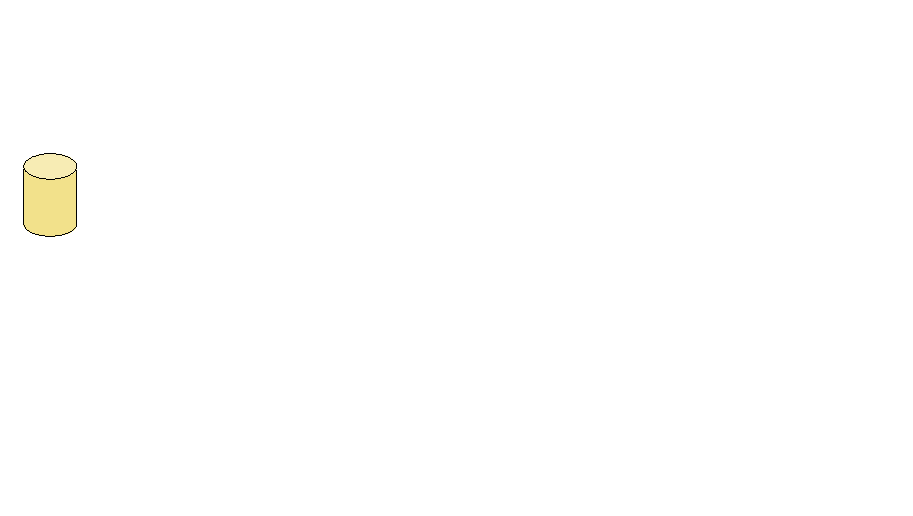
\includegraphics[width=\textwidth]{proposed_architecture.eps}
		\caption{Proposed Architecture}%
		\label{fig:proposed_architecture}
	\end{figure}

	The software architecture will probably be developed in C++, but other
	languages such as Python may also be employed. The following lists the main
	design goals of the proposed architecture:

	\begin{enumerate}

		\item\label{goal:flexibile}

			Be flexible and extendible.

		\item\label{goal:guarantee_trajectory}

			Guarantee collision free trajectories.

	\end{enumerate}

	Goal~\ref{goal:flexibile} may be achieved by adhering to good coding
	practices, whereas Goal~\ref{goal:guarantee_trajectory} is more algorithmic
	in nature. It requires a good understanding and implementation of algorithms
	and methods such as those reported in this literature study.

	One point that may be worth exploring is the generation of an architecture
	that can adapt to different \gls{cdpr} structures. This will require the
	creation of a configuration file format that describes the topology of the
	robot. This is represented as the ``Robot Topology'' database in
	Figure~\ref{fig:proposed_architecture} and may help to further
	Goal~\ref{goal:flexibile}. Furthermore, the steps denoted in
	Figure~\ref{fig:proposed_architecture} should be designed as separate
	modules that adhere to a predetermined interface. This will enable them to
	be interchanged with other modules and algorithms during the progression of
	the thesis.

	With a knowledge of the topology, the architecture will be capable of
	building an internal representation of the robot. Using a type of
	semi-algebraic representation such as those discussed in
	Section~\ref{sec:semi_algebraic_representation_of_bodies} seems to be the
	most promising at present, but other representations may also be
	investigated. A similar approach can be used to model obstacles in the
	world.

	It may be expensive to evaluate the workspace of the robot using methods
	from Section~\ref{sec:continuous_workspace_determination}, but may be worth
	investigating such an approach. Persisting the workspace representation
	could save time in future calculations. The main potential benefit of
	modelling the workspace is that it could potentially limit the total
	configuration space that needs to be searched for a path.

	$\configurationspace$ should ideally be sampled in such a way as to allow
	multiple queries, thereby improving the overall response time of the
	architecture. To this end, $\configurationspace_{\freeregion}$ will be
	represented in a topological graph $\topologicalgraph$ that can be used with
	classical discrete graph search algorithms. Depending on the path planning
	algorithm used, it might be necessary to smooth the calculated path. This is
	currently envisioned as a step after the path has been calculated and may be
	implemented by following methods similar to that described in
	Section~\ref{sec:smoothing_random_paths}.

	The path generated by the architecture should ideally not yet encode any
	timing of the final trajectory. The ``Generate Trajectory'' step of
	Figure~\ref{fig:proposed_architecture} should instead translate the path
	into a time-dependent trajectory. Methods from
	Chapter~\ref{sec:trajectory_generation} may be used in this step. Finally,
	it may be necessary to employ post-processing methods discussed in
	Section~\ref{sec:trajectory_scaling} to meet dynamic requirements of the
	trajectory.

	\subsection{Projected Work Progression}%
	\label{sec:projected_work_progression}

		Initial work will be of a theoretical nature. The main expected steps is
		documented below:

		\begin{enumerate}

			\item

				At first, the planar case will be studied. Methods for
				generating translational motions will be investigated.

			\item

				Next, orientation trajectories of the
				$\specialOrthonormalGroup{2}$ group will be studied.

			\item

				These trajectories will be combined to investigate general
				planar trajectories in the $\specialEuclideanGroup{2}$ group.

			\item

				When the work on planar trajectories has been studied, it will
				be generalised into the three-dimensional case. At first, these
				trajectories will again only be translational.

			\item

				When translational trajectories are working, three-dimensional
				rotations of the $\specialOrthonormalGroup{3}$ group will be
				investigated.

			\item

				Finally, the most general three-dimensional case of trajectories
				in the $\specialEuclideanGroup{3}$ group will be studied.

		\end{enumerate}

		Once theoretical work has been done, experimental validation will be
		performed on a real robot. An ACROBOT with a $1m^3$ volume  will be
		used. This robot is shown in Figure~\ref{fig:acrobot}. There is also the
		possibility of experimenting on a CAROCA, with volume
		$7m\times4m\times3.5m$.

		\begin{figure}[hb]
			\centering
			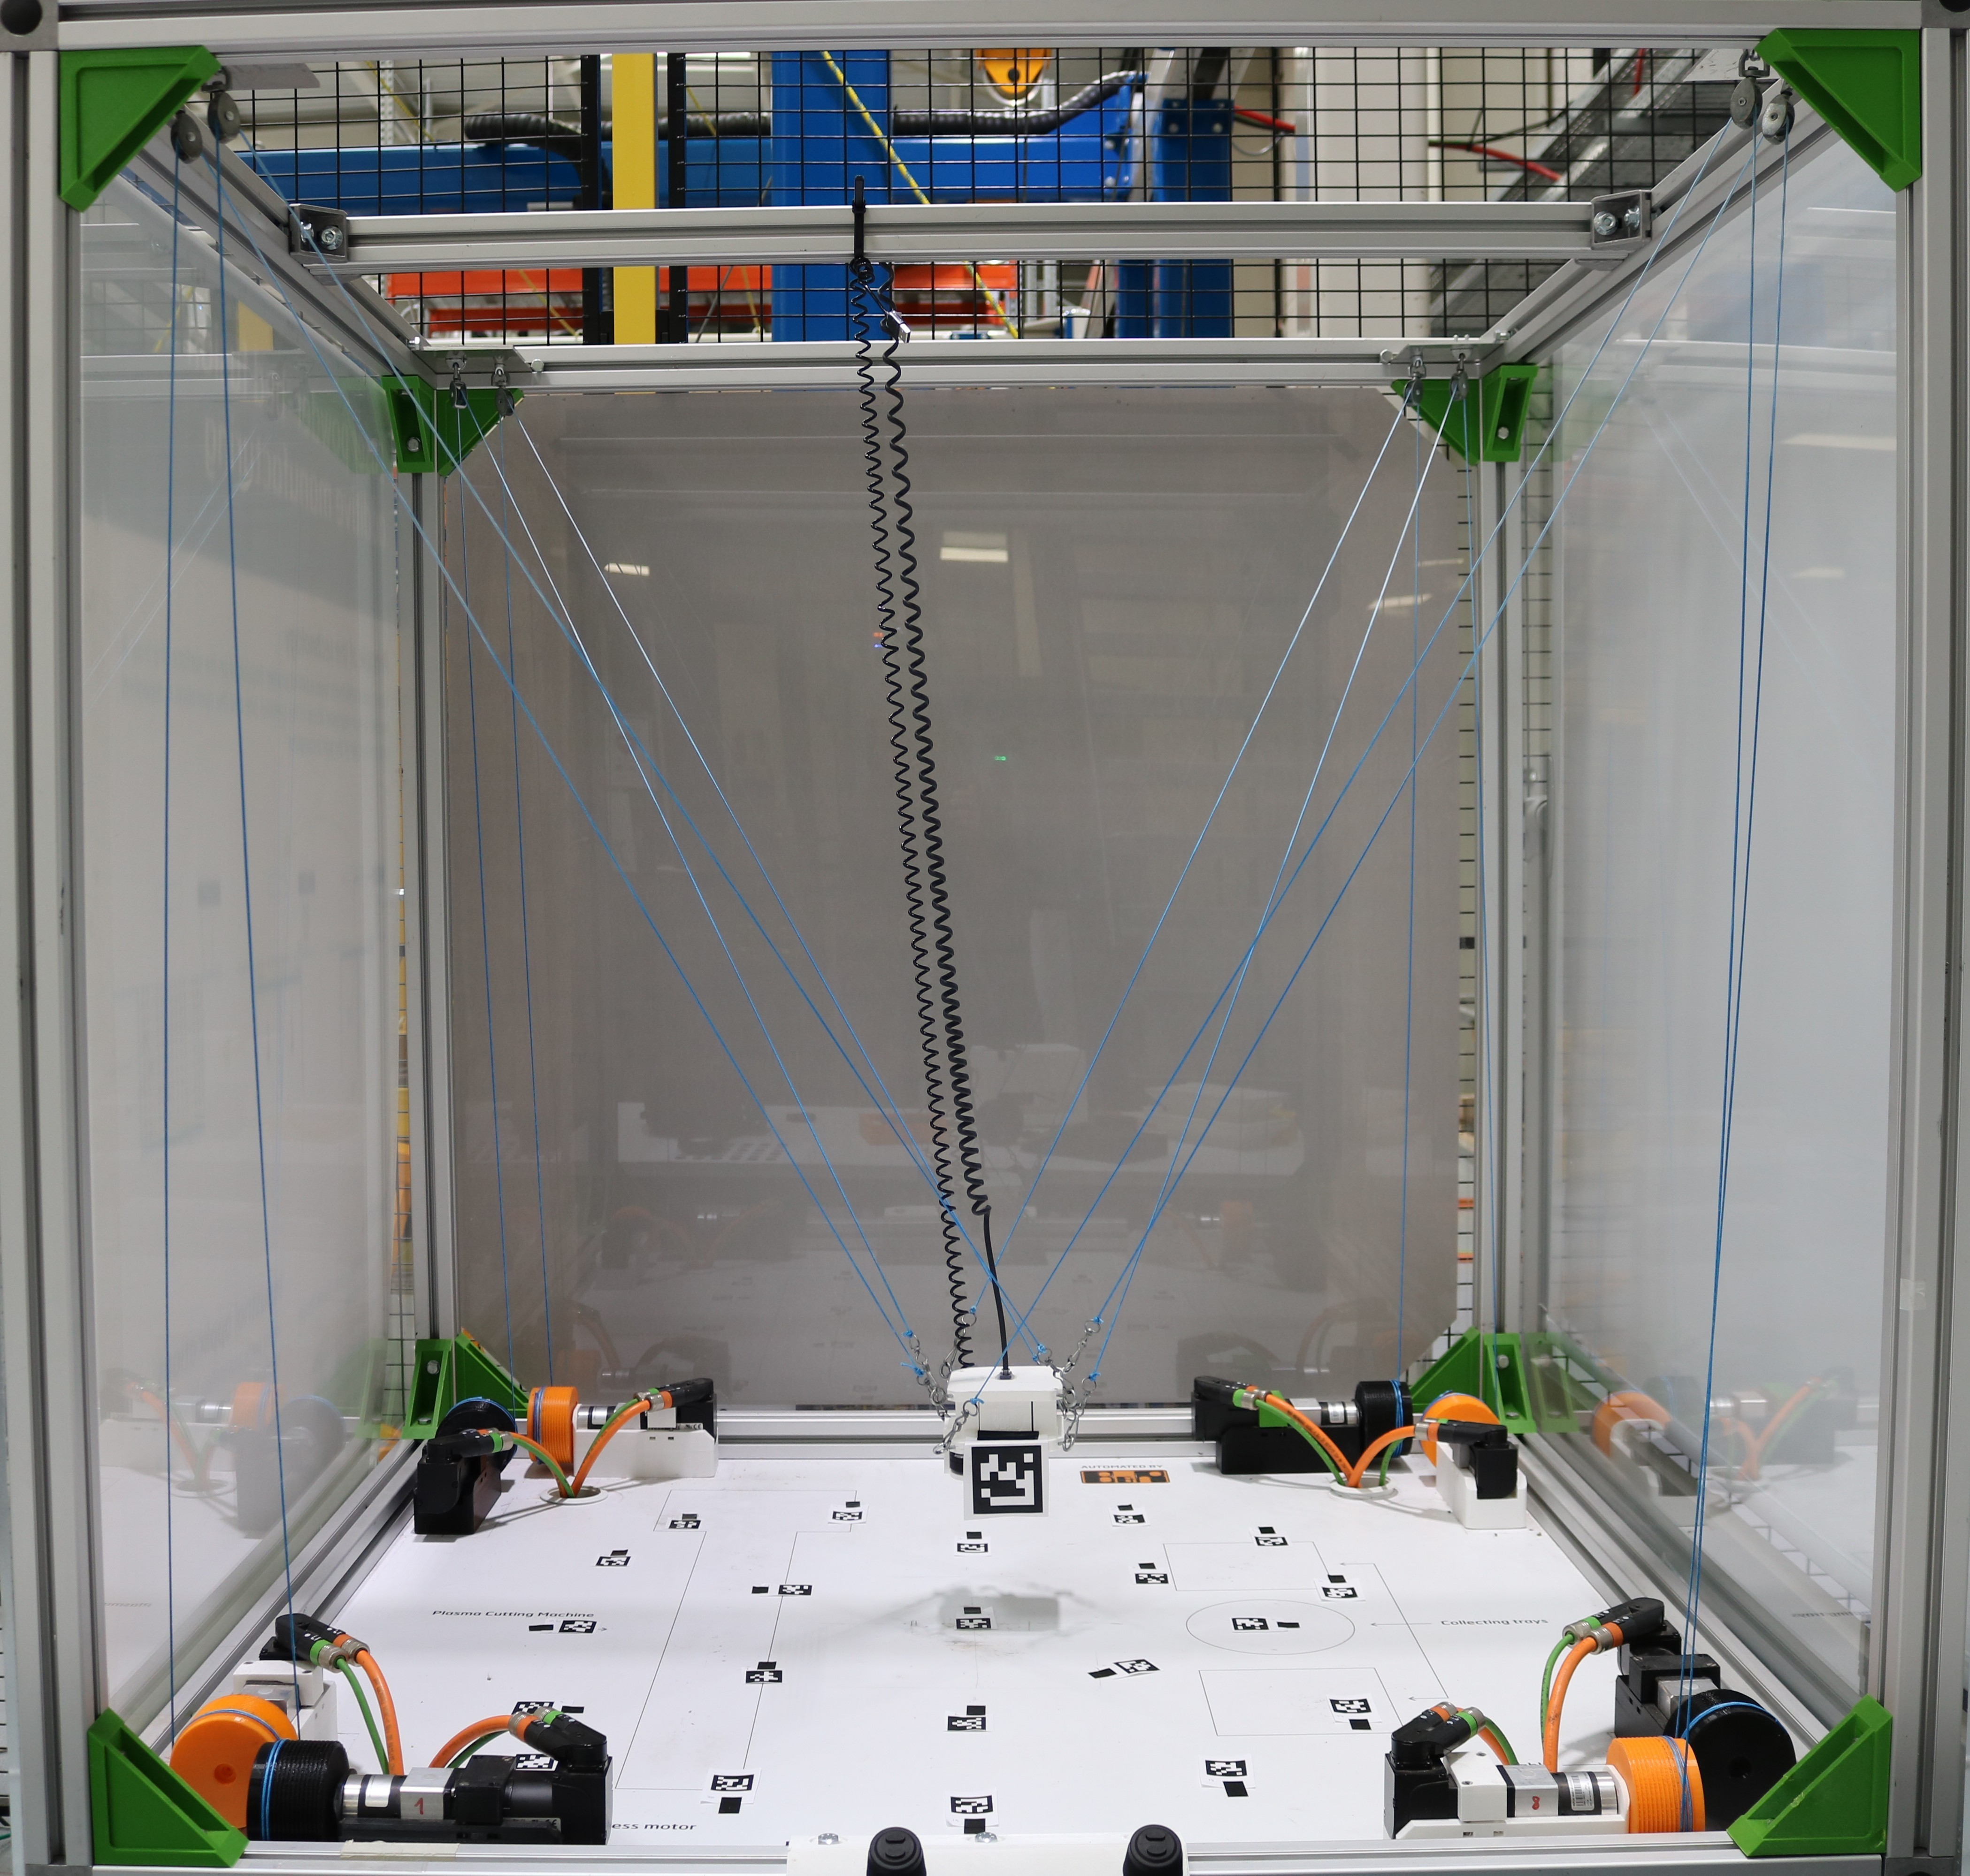
\includegraphics[width=0.5\textwidth]{acrobotHD}
			\caption{ACROBOT}
			\label{fig:acrobot}
		\end{figure}
